\documentclass[10pt,a4paper]{article}
\usepackage[utf8]{inputenc}
\usepackage{amsmath}
\usepackage{amsfonts}
\usepackage{amssymb}
\usepackage{listings}
\usepackage{graphicx}
\usepackage{caption}
\usepackage{subcaption}
\usepackage{float}
\lstset{showstringspaces=false,
		breaklines=true,
		postbreak=\raisebox{0ex}[0ex][0ex]{\ensuremath{\hookrightarrow\space}}}
    	
\begin{document}
\title{Intelligent Systems Assignment 3}
\author{Wessel Becker (1982362) \& Sander ten Hoor (2318555)}
\maketitle

\section{Matlab Code}
The following code was created for edge detection and boundary detection.

\subsection{simpleDifferentiation.m}
\lstinputlisting[language=Matlab]{./edgedetection/simpleDifferentiation.m}

\subsection{robert.m}
\lstinputlisting[language=Matlab]{./edgedetection/robert.m}

\subsection{sobel.m}
\lstinputlisting[language=Matlab]{./edgedetection/sobel.m}

\subsection{prewitt.m}
\lstinputlisting[language=Matlab]{./edgedetection/prewitt.m}

\subsection{boundaryExtraction.m}
\lstinputlisting[language=Matlab]{./edgedetection/boundaryExtraction.m}\label{list:boundaryExtraction}

\subsection{displayCannyEdgeDetectionSpecific.m}
\lstinputlisting[language=Matlab]{./edgedetection/displayCannyEdgeDetectionSpecific.m}

\section{Edge Detection}
While all the results suffer from noise, the Simple Differentiation and the Roberts algorithm become nearly unrecognisable, while the others still show clear lines.

\section{Boundary Extraction}
For exercise 2.2 a simple boundary extractor was build as can be found in the code listings \ref{list:boundaryExtraction}. This very simple boundary extractor can be run with a variable threshold for hit detection. And works by first eroding anything that could be the inside of a shape by doing an erosion with a 3 * 3 structuring element with the origo in the center. This will erode any pixel that is not surrounded by other accepted pixels but is accepted, or in other words the boundaries. If we then subtract this image from our original binary image of accepted values we are left with the pixels we eroded before or in other words the boundaries as seen in figure \ref{fig:boundary_extraction}.

\section{Canny Edge Detection}
Exercise 2.3 asked us to analyse the impact of noise, more specifically Gaussian noise, on the Canny Edge Detection algorithm. We also consider the influence of some of the tuning variables for the algorithm, most importantly the sigma variable, further referred to as s, which is the standard deviation for the Gaussian blur filter. We will also take a  look at the influence of changing the threshold values for the acceptance of weak and strong edges. This variable will be referred to as t and it is represented as a factor of the weak edge threshold and the strong edge threshold respectively.

It is expected that when the Gaussian noise is increased the edge detection algorithm will start to pick more false edges. It is also expected that increasing s and therefore also the size of the Gaussian filter will reduce the amount of false edges when the level of noise is increased, however probably at some cost to the amount of true edges being detected.

Further expected is, that choosing a lower value for the weak edge threshold will increase the amount of weaker edges connected to strong edges that is detected, but increasing the amount of false positives as it gets lower as well, especially in an image with more Gaussian noise. 

And lastly we expect that the lower the value chosen for the strong edge threshold the more edges we will find in general, however making this value to low should lead to many false positives for the edges especially in images with a lot of noise.

\subsection{No noise}
Figure \ref{fig:cany_no_noise_default} is the result of the Canny algorithm, with the chest image as input and the settings at default. When the smoothing is decreased (Figure \ref{fig:cany_no_noise_low_s}) the number of detected edges increases as a result of a less smooth image. When the smoothing is higher than the default (Figure \ref{fig:cany_no_noise_high_s}) there are less edges detected. Similar, predictable effects are obtained when changing the thresholds. 

\subsection{Medium noise}
A notable difference between the no noise images and medium noise images is the decreased number of lines found with less smoothing. Figure \ref{fig:cany_no_noise_default} and figure \ref{fig:m_noise_def} are produced using the same settings, but the latter has some noise but produces less edges. Same goes for figure \ref{fig:cany_no_noise_low_s} and \ref{fig:m_noise_l_sigma_sqr1}. This could be because of the noise interfering with the existing edges, which results in no longer meeting the weak or strong edge thresholds. The difference between figure \ref{fig:no_noise_t_00625_00781} (no noise) and figure \ref{fig:m_noise_sens_h_thres} (medium noise), where the latter shows a lot more edges due to the lowered threshold, seems to support this.

Figures \ref{fig:m_noise_def} and \ref{fig:m_noise_h_sigma_sqr3} both have a close resemblance to the original figure \ref{fig:cany_no_noise_default}.

\subsection{Heavy noise}
All the images with heavy noise show more edges than the no noise and the medium images, as expected. Increased smoothing does indeed help with detecting less false positives, but it also fails to show some true edges (figure \ref{fig:h_noise_h_sigma_sqr3}). This image is the closest to the original.

\subsection{Conclusion}
The expected behavior as a consequence of changes in s and t did indeed happen.

The differences between no noise, medium noise and heavy noise become increasingly difficult to fix as the noise level increases. Smoothing produces images that are more or less similar to the no noise image with default settings (figure \ref{fig:cany_no_noise_default}, but details are lost and the result is never quite te same. Nonetheless, the increased smoothing seems to be the most successful when noise levels increase. 

\section{Surround Suppression}
Surround suppression is a way of enhancing contours and region boundaries in images with texture. This works in combination with the Canny Edge Detection algorithm.

\subsection{kanizsa}
The kanizsa image is a binary image, meaning that the usage of surround suppression will not impact the edge detection on this image greatly.
For an initial comparison, $\alpha$ = 2, K1 = 1 and K2 = 4 was used with Isotropic (L-infinity, L1 and L2 norms) and Anisotropic.

\section{Work done}

\section{Edge Detection images}
\subsection{Simple Differentiation}

\begin{figure}
  \centering
  
  \begin{subfigure}{.5\textwidth}
    \centering
    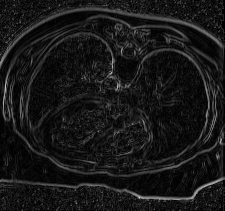
\includegraphics[width=.9\textwidth]{./edgedetection/images/sd_no_noise}
    \caption{Simple Differentiation, no noise}
    \label{fig:sd_no_noise}
  \end{subfigure}%
  \begin{subfigure}{.5\textwidth}
    \centering
    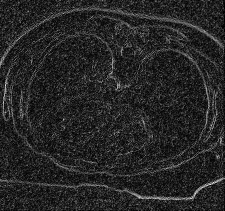
\includegraphics[width=.9\textwidth]{./edgedetection/images/sd_001_noise}
    \caption{Simple Differentiation, Gaussian noise with variance = 0.001}
    \label{fig:sd_001}
  \end{subfigure}\\%
  \begin{subfigure}{.5\textwidth}
    \centering
    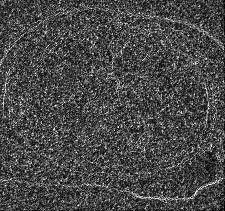
\includegraphics[width=.9\textwidth]{./edgedetection/images/sd_005_noise}
    \caption{Simple Differentiation, Gaussian noise with variance = 0.005}
    \label{fig:sd_005}
  \end{subfigure}%
  
\end{figure}

\subsection{Roberts}
\begin{figure}
  \centering
    \makebox[\textwidth]{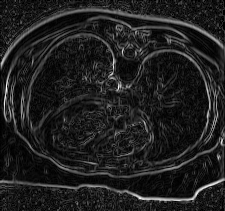
\includegraphics{./edgedetection/images/robert_no_noise}} \\
  \caption{Roberts, no noise}
  \label{fig:robert_no_noise}
\end{figure}

\begin{figure}
  \centering
    \makebox[\textwidth]{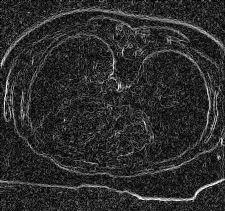
\includegraphics{./edgedetection/images/robert_001_noise}} \\
  \caption{Roberts, Gaussian noise with variance = 0.001}
  \label{fig:robert_001}
\end{figure}

\begin{figure}
  \centering
    \makebox[\textwidth]{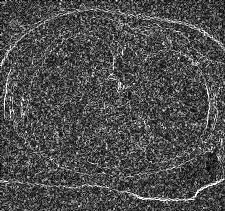
\includegraphics{./edgedetection/images/robert_005_noise}} \\
  \caption{Roberts, Gaussian noise with variance = 0.005}
  \label{fig:robert_005}
\end{figure}

\subsection{Sobel}
\begin{figure}
  \centering
    \makebox[\textwidth]{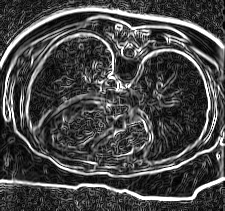
\includegraphics{./edgedetection/images/sobel_no_noise}} \\
  \caption{Sobel, no noise}
  \label{fig:sobel_no_noise}
\end{figure}

\begin{figure}
  \centering
    \makebox[\textwidth]{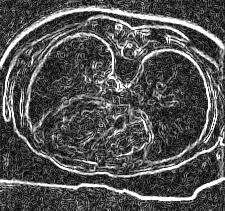
\includegraphics{./edgedetection/images/sobel_001_noise}} \\
  \caption{Sobel, Gaussian noise with variance = 0.001}
  \label{fig:sobel_001}
\end{figure}

\begin{figure}
  \centering
    \makebox[\textwidth]{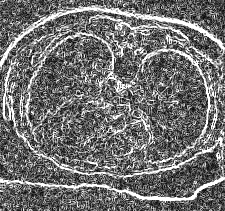
\includegraphics{./edgedetection/images/sobel_005_noise}} \\
  \caption{Sobel, Gaussian noise with variance = 0.005}
  \label{fig:sobel_005}
\end{figure}

\subsection{Prewitt}

\begin{figure}
  \centering
    \makebox[\textwidth]{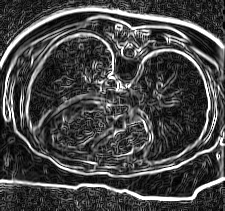
\includegraphics{./edgedetection/images/prewitt_no_noise}} \\
  \caption{Prewitt, no noise}
  \label{fig:prewitt_no_noise}
\end{figure}

\begin{figure}
  \centering
    \makebox[\textwidth]{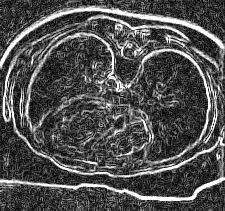
\includegraphics{./edgedetection/images/prewitt_001_noise}} \\
  \caption{Prewitt, Gaussian noise with variance = 0.001}
  \label{fig:prewitt_001}
\end{figure}

\begin{figure}
  \centering
    \makebox[\textwidth]{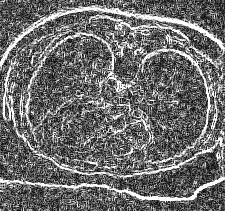
\includegraphics{./edgedetection/images/prewitt_005_noise}} \\
  \caption{Prewitt, Gaussian noise with variance = 0.005}
  \label{fig:prewitt_005}
\end{figure}

\section{Boundary detection}
\begin{figure}[H]
  \centering
    \makebox[\textwidth]{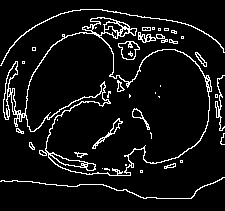
\includegraphics[width=.9\textwidth]{./edgedetection/boundary_extraction/boundary_extraction}} \\
  \caption{Scatter, n = 0.1, 2 prototypes}
  \label{fig:n01_k2}
\end{figure}

\section{Canny images}
\subsection{No noise}
\begin{figure}[H]
  \centering
  
  \begin{subfigure}{.5\textwidth}
    \centering
    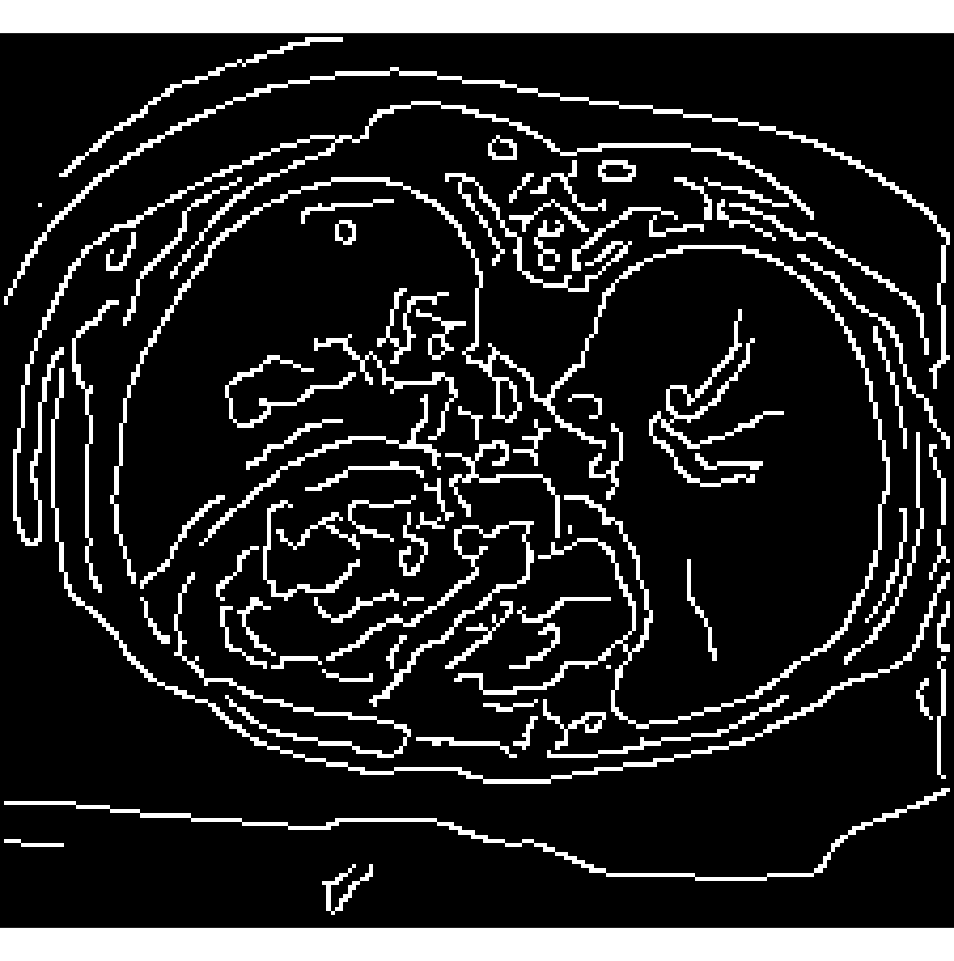
\includegraphics[width=.9\textwidth]{./edgedetection/canny_no_noise/no_noise_t_00625_01562}
    \caption{No noise, t = [0.0625, 0.1562], s = sqrt(2)}
    \label{fig:cany_no_noise_default}
  \end{subfigure}%
  \begin{subfigure}{.5\textwidth}
    \centering
    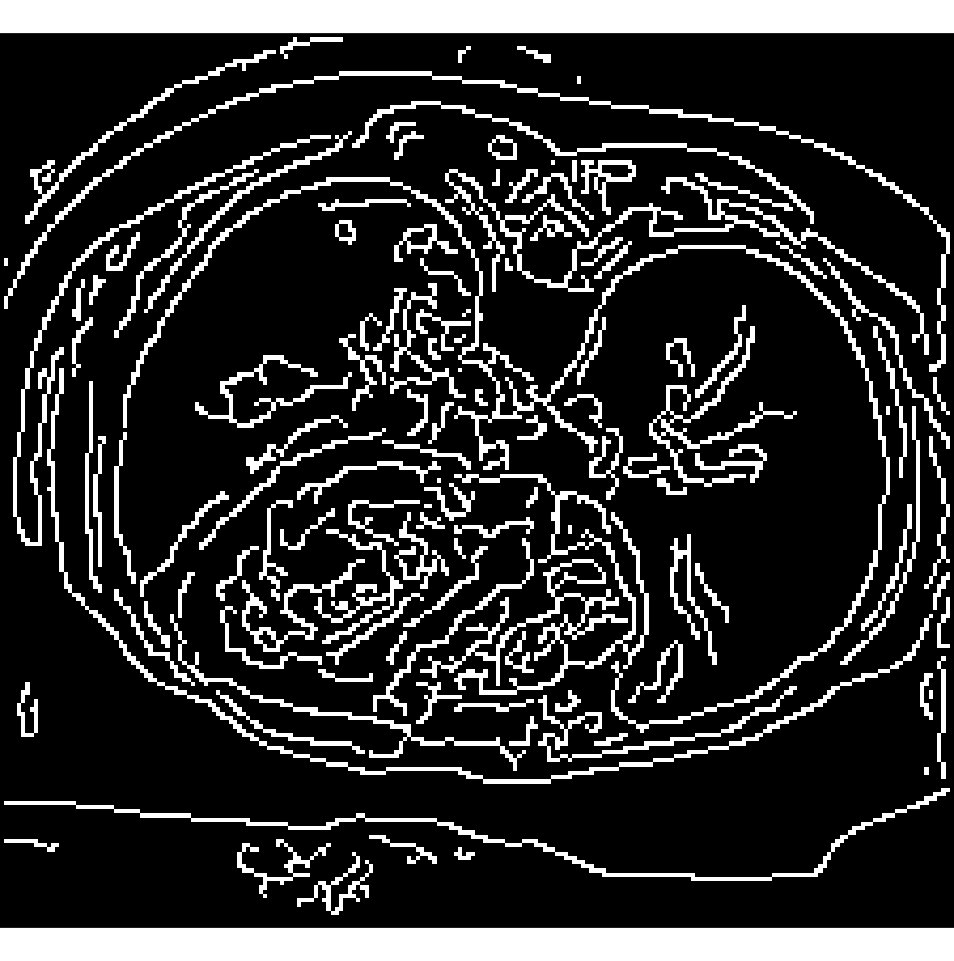
\includegraphics[width=.9\textwidth]{./edgedetection/canny_no_noise/no_noise_s_srt_1}
    \caption{No noise, t = [0.0625, 0.1562], s = sqrt(1)}
    \label{fig:cany_no_noise_low_s}
  \end{subfigure}\\%
  \begin{subfigure}{.5\textwidth}
    \centering
    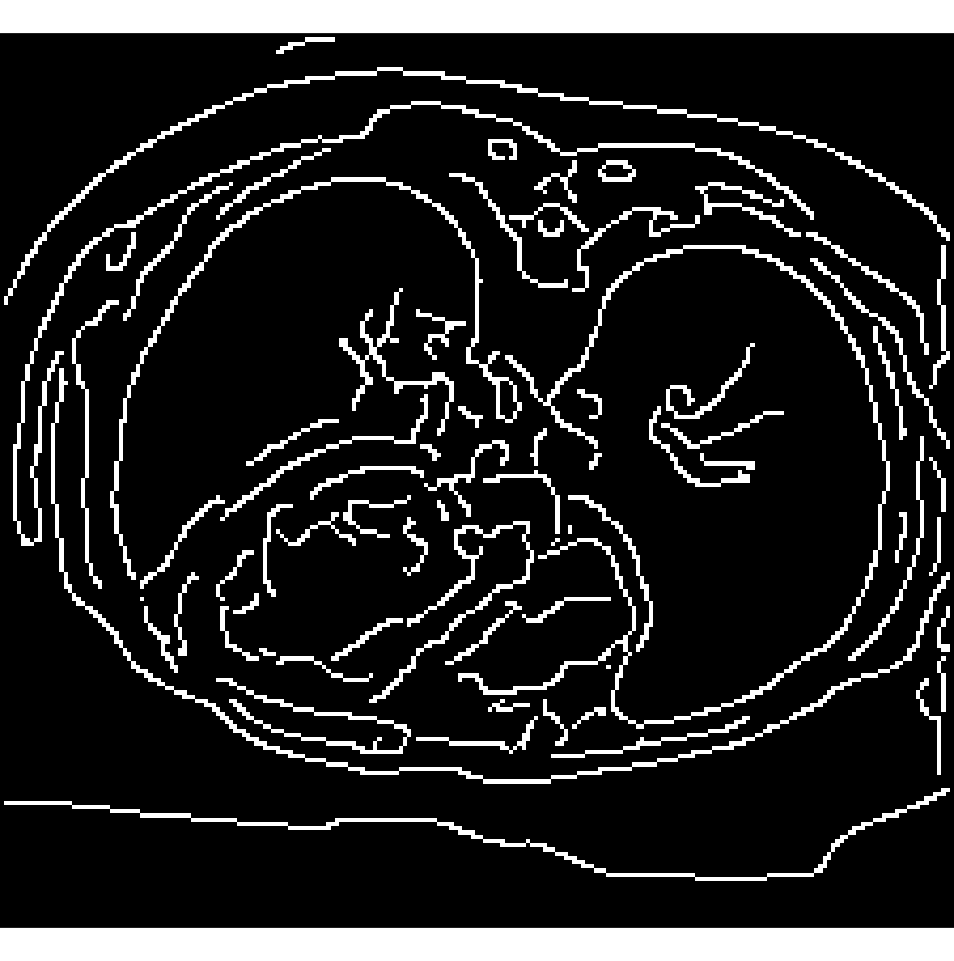
\includegraphics[width=.9\textwidth]{./edgedetection/canny_no_noise/no_noise_s_srt_3}
    \caption{No noise, t = [0.0625, 0.1562], s = sqrt(3)}
    \label{fig:cany_no_noise_high_s}
  \end{subfigure}%
  \begin{subfigure}{.5\textwidth}
    \centering
    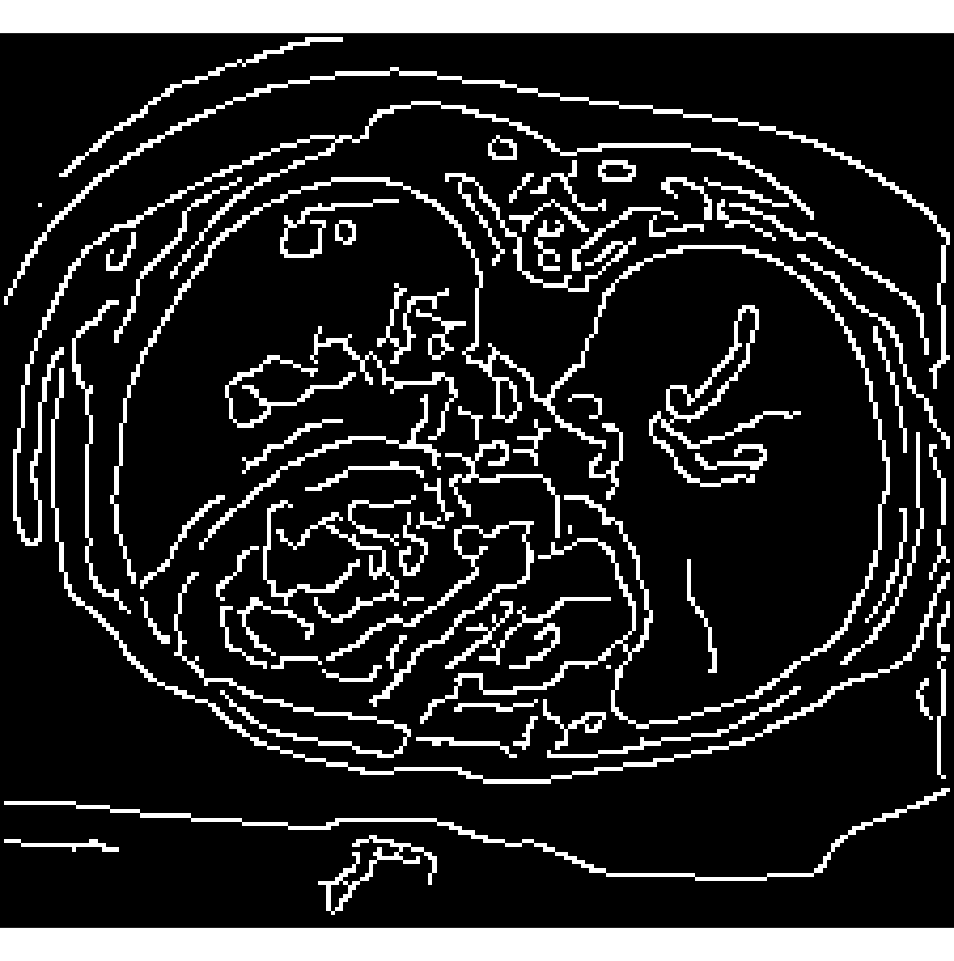
\includegraphics[width=.9\textwidth]{./edgedetection/canny_no_noise/no_noise_t_003125_01562}
    \caption{No noise, t = [0.03125, 0.1562], s = sqrt(2)}
    \label{fig:cany_no_noise_low_low_t}
  \end{subfigure}%
  
\end{figure}

\begin{figure}[H]
  \centering
  
  \begin{subfigure}{.5\textwidth}
    \centering
    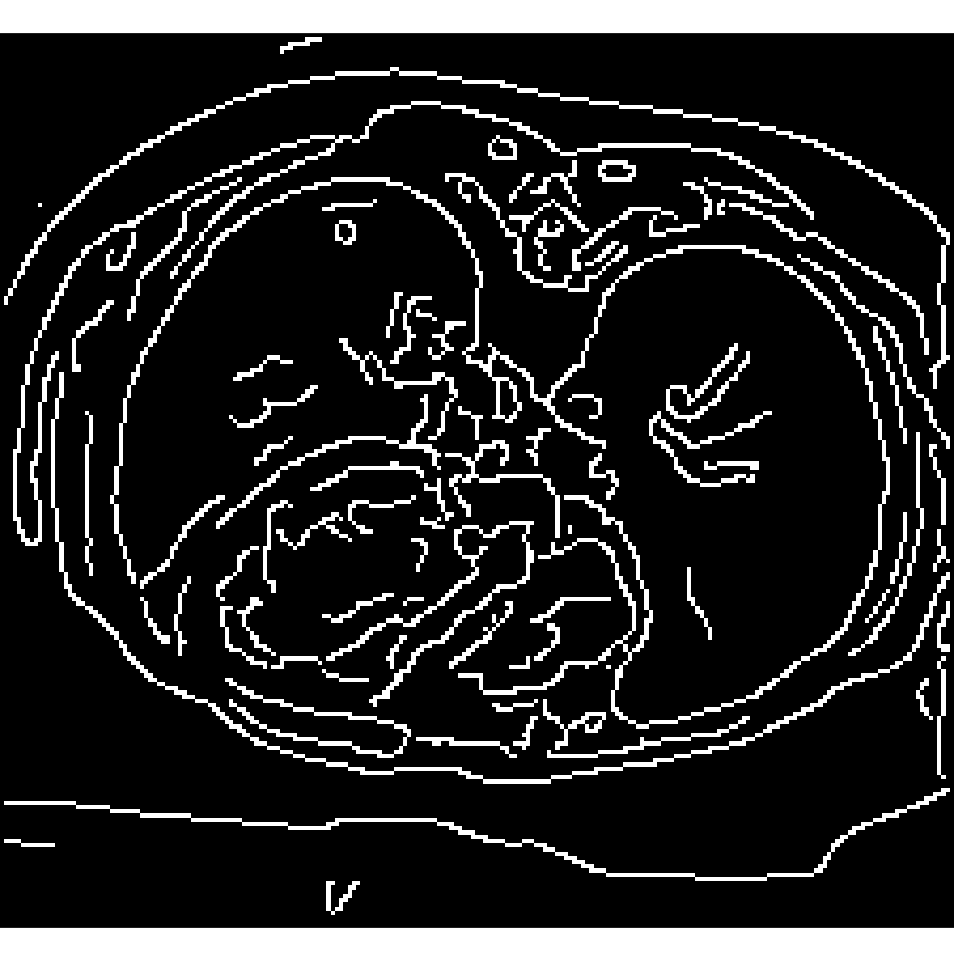
\includegraphics[width=.9\textwidth]{./edgedetection/canny_no_noise/no_noise_t_009375_01562}
    \caption{No noise, t = [0.09375, 0.1562], s = sqrt(2)}
    \label{fig:cany_no_noise_high_low_t}
  \end{subfigure}%
  \begin{subfigure}{.5\textwidth}
    \centering
    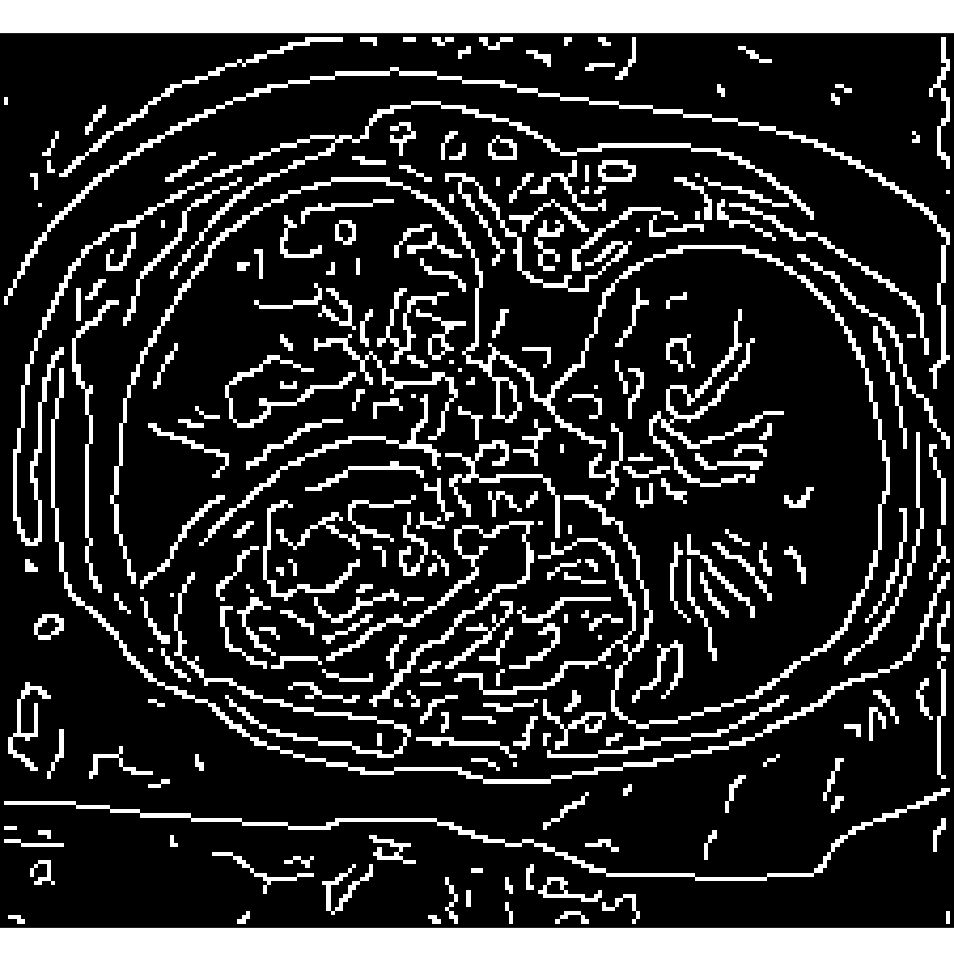
\includegraphics[width=.9\textwidth]{./edgedetection/canny_no_noise/no_noise_t_00625_00781}
    \caption{No noise, t = [0.0625, 0.0781], s = sqrt(2)}
    \label{fig:no_noise_t_00625_00781}
  \end{subfigure}\\%
  \begin{subfigure}{.5\textwidth}
    \centering
    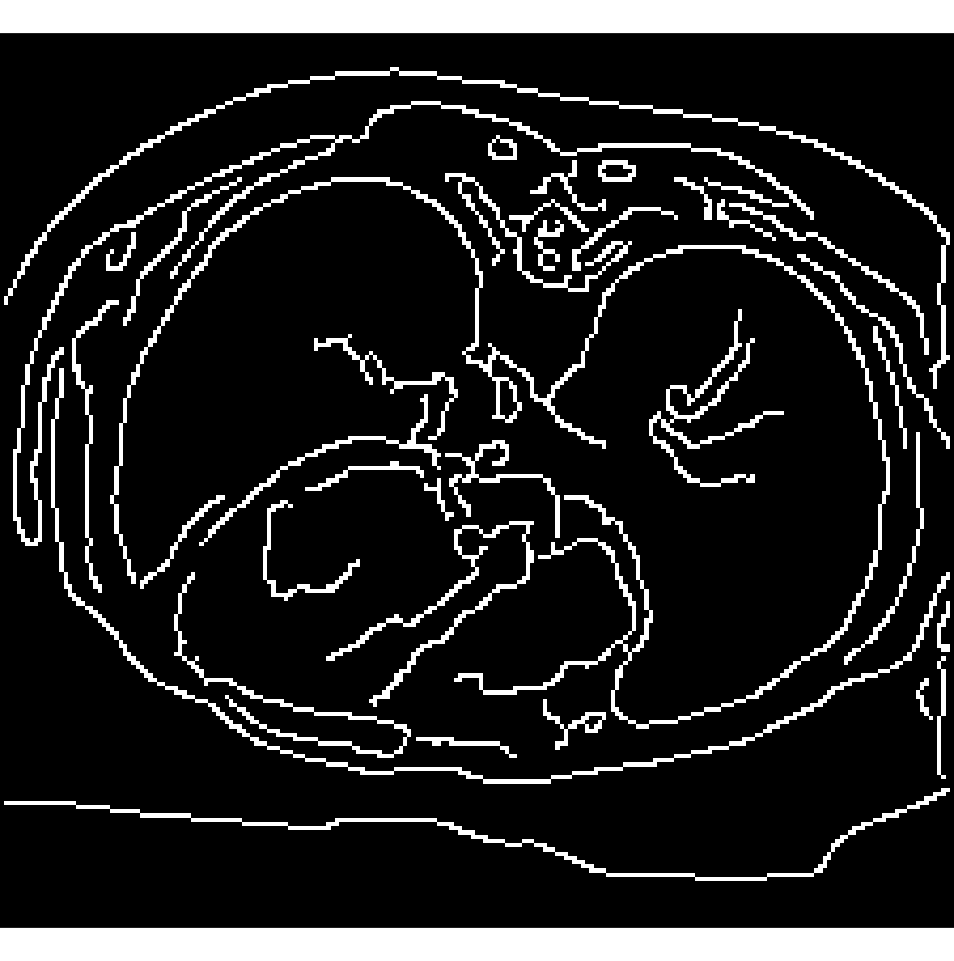
\includegraphics[width=.9\textwidth]{./edgedetection/canny_no_noise/no_noise_t_00625_02343}
    \caption{No noise, t = [0.0625, 0.2343], s = sqrt(2)}
    \label{fig:cany_no_noise}
  \end{subfigure}%
  
\end{figure}
\subsection{Medium noise}
\begin{figure}[H]
  \centering
  
  \begin{subfigure}{.5\textwidth}
    \centering
    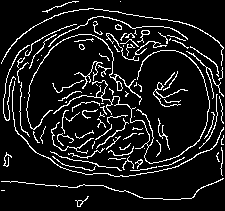
\includegraphics[width=.9\textwidth]{./edgedetection/medium_noise/m_noise_def}
    \caption{Medium noise, default}
    \label{fig:m_noise_def}
  \end{subfigure}%
  
  \begin{subfigure}{.5\textwidth}
    \centering
    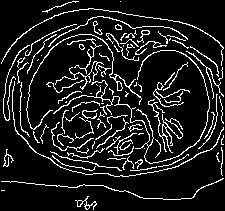
\includegraphics[width=.9\textwidth]{./edgedetection/medium_noise/m_noise_sens_l_thres}
    \caption{Medium noise, sensitive, low threshold}
    \label{fig:m_noise_sens_l_thres}
  \end{subfigure}\\%
  
  \begin{subfigure}{.5\textwidth}
    \centering
    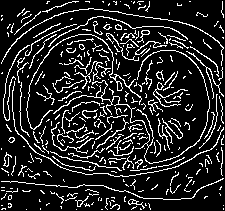
\includegraphics[width=.9\textwidth]{./edgedetection/medium_noise/m_noise_sens_h_thres}
    \caption{Medium noise, sensitive, high threshold}
    \label{fig:m_noise_sens_h_thres}
  \end{subfigure}%
  
  \begin{subfigure}{.5\textwidth}
    \centering
    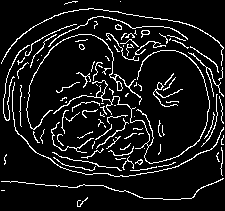
\includegraphics[width=.9\textwidth]{./edgedetection/medium_noise/m_noise_insens_l_thres}
    \caption{Medium noise, insensitive, low threshold}
    \label{fig:m_noise_insens_l_thres}
  \end{subfigure}\\%
  
  \begin{subfigure}{.5\textwidth}
    \centering
    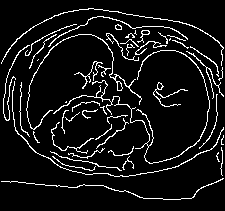
\includegraphics[width=.9\textwidth]{./edgedetection/medium_noise/m_noise_insens_h_thres}
    \caption{Medium noise, insensitive, high threshold}
    \label{fig:m_noise_insens_h_thres}
  \end{subfigure}%
  
    \begin{subfigure}{.5\textwidth}
    \centering
    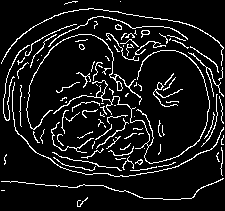
\includegraphics[width=.9\textwidth]{./edgedetection/medium_noise/m_noise_insens_l_thres}
    \caption{Medium noise, low sigma, sqrt(1)}
    \label{fig:m_noise_insens_l_thres}
  \end{subfigure}\\%
  
  \begin{subfigure}{.5\textwidth}
    \centering
    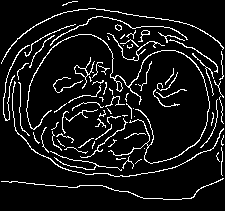
\includegraphics[width=.9\textwidth]{./edgedetection/medium_noise/m_noise_h_sigma_sqr3}
    \caption{Medium noise, high sigma, sqrt(3)}
    \label{fig:m_noise_h_sigma_sqr3}
  \end{subfigure}%
  
\end{figure}


\subsection{Heavy noise}
\begin{figure}[H]
  \centering
  
  \begin{subfigure}{.5\textwidth}
    \centering
    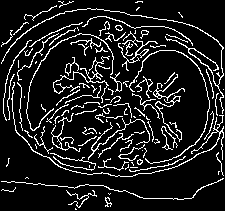
\includegraphics[width=.9\textwidth]{./edgedetection/heavy_noise/h_noise_def}
    \caption{Heavy noise, t = [0.0625, 0.1562], s = sqrt(2)}
    \label{fig:h_noise_def}
  \end{subfigure}%
      \begin{subfigure}{.5\textwidth}
    \centering
    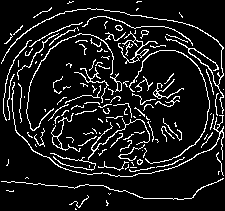
\includegraphics[width=.9\textwidth]{./edgedetection/heavy_noise/h_noise_insens_l_thres}
    \caption{Heavy noise, t = [0.0625, 0.1562], s = sqrt(1)}
    \label{fig:h_noise_insens_l_thres}
  \end{subfigure}\\%
    \begin{subfigure}{.5\textwidth}
    \centering
    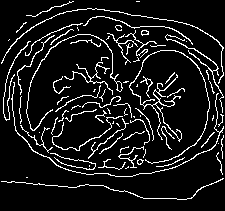
\includegraphics[width=.9\textwidth]{./edgedetection/heavy_noise/h_noise_h_sigma_sqr3}
    \caption{Heavy noise, t = [0.0625, 0.1562], s = sqrt(3)}
    \label{fig:h_noise_h_sigma_sqr3}
  \end{subfigure}%
  \begin{subfigure}{.5\textwidth}
    \centering
    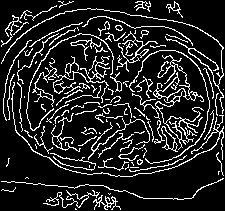
\includegraphics[width=.9\textwidth]{./edgedetection/heavy_noise/h_noise_sens_l_thres}
    \caption{Heavy noise, t = [0.03125, 0.1562], s = sqrt(2)}
    \label{fig:h_noise_sens_l_thres}
  \end{subfigure}\\%
\end{figure}

\begin{figure}[H]
  \centering
  
	\begin{subfigure}{.5\textwidth}
    \centering
    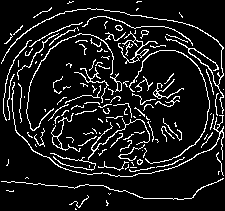
\includegraphics[width=.9\textwidth]{./edgedetection/heavy_noise/h_noise_insens_l_thres}
    \caption{Heavy noise, t = [0.09375, 0.1562], s = sqrt(2)}
    \label{fig:h_noise_insens_l_thres}
  \end{subfigure}\\%
    \begin{subfigure}{.5\textwidth}
    \centering
    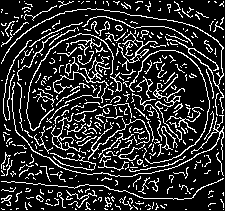
\includegraphics[width=.9\textwidth]{./edgedetection/heavy_noise/h_noise_sens_h_thres}
    \caption{Heavy noise, t = [0.0625, 0.0781], s = sqrt(2)}
    \label{fig:h_noise_sens_h_thres}
  \end{subfigure}%
  \begin{subfigure}{.5\textwidth}
    \centering
    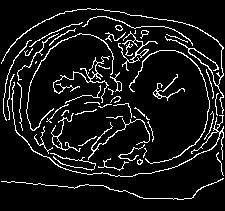
\includegraphics[width=.9\textwidth]{./edgedetection/heavy_noise/h_noise_insens_h_thres}
    \caption{Heavy noise, t = [0.0625, 0.2343], s = sqrt(2)}
    \label{fig:h_noise_insens_h_thres}
  \end{subfigure}%
  
\end{figure}



\section{Surround suppression images}
\subsection{kanisza}
\begin{figure}[H]
  \centering

\begin{subfigure}{.7\textwidth}
    \centering
    
\includegraphics[width=.9\textwidth]{./canny/kanizsa}
    \caption{Original kanizsa image}
    \label{fig:kanizsa}
  \end{subfigure}%  

\end{figure}
\subsubsection{kanisza, alpha = 2}
% Kanizsa, alpha = 2
\begin{figure}[H]
  \centering

\begin{subfigure}{.7\textwidth}
    \centering
    
\includegraphics[width=.9\textwidth]{./canny/kanizsa}
    \caption{Original kanizsa image}
    \label{fig:kanizsa}
  \end{subfigure}%  
  
    \begin{subfigure}{.7\textwidth}
    \centering
    
\includegraphics[width=.9\textwidth]{./canny/kanizsa_LINF_a2_k11_k24}
    \caption{kanizsa, Isotropic L-infinity norm. $\alpha$ = 2, K1 = 1, K2 = 4}
    \label{fig:kanizsa_LINF_a2_k11_k24}
  \end{subfigure}%

\end{figure}

\begin{figure}[H]
\centering

  \begin{subfigure}{.7\textwidth}
    \centering
    
\includegraphics[width=.9\textwidth]{./canny/kanizsa_L1_a2_k11_k24}
    \caption{kanizsa, Isotropic L1 norm. $\alpha$ = 2, K1 = 1, K2 = 4}
    \label{fig:kanizsa_L1_a2_k11_k24}
  \end{subfigure}%
  
  \begin{subfigure}{.7\textwidth}
    \centering
    
\includegraphics[width=.9\textwidth]{./canny/kanizsa_L2_a2_k11_k24}
    \caption{kanizsa, Isotropic L2 norm. $\alpha$ = 2, K1 = 1, K2 = 4}
    \label{fig:kanizsa_L2_a2_k11_k24}
  \end{subfigure}\\%
 \end{figure}

\begin{figure}[H]
\centering 
  \begin{subfigure}{.7\textwidth}
    \centering
    
\includegraphics[width=.9\textwidth]{./canny/kanizsa_ANISO_a2_k11_k24}
    \caption{kanizsa, Anisotropic. $\alpha$ = 2, K1 = 1, K2 = 4}
    \label{fig:kanizsa_ANISO_a2_k11_k24}
  \end{subfigure}%
  
\end{figure}
\subsubsection{kanisza, alpha = 4}
% Kanizsa, alpha = 2
\begin{figure}[H]
  \centering
  
    \begin{subfigure}{.7\textwidth}
    \centering
    
\includegraphics[width=.9\textwidth]{./canny/kanizsa_LINF_a4_k11_k24}
    \caption{kanizsa, Isotropic L-infinity norm. $\alpha$ = 4, K1 = 1, K2 = 4}
    \label{fig:kanizsa_LINF_a4_k11_k24}
  \end{subfigure}%

\end{figure}

\begin{figure}[H]
\centering

  \begin{subfigure}{.7\textwidth}
    \centering
    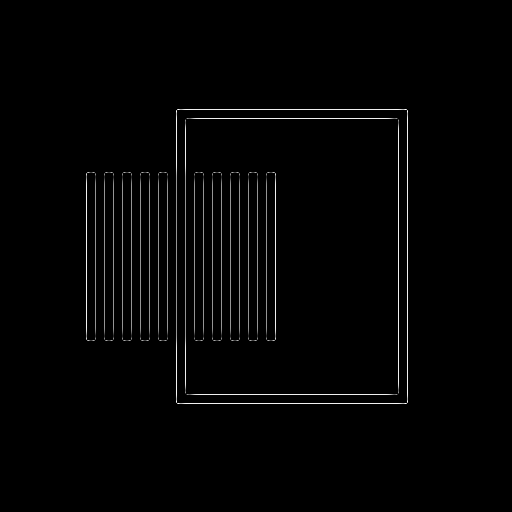
\includegraphics[width=.9\textwidth]{./canny/kanizsa_L1_a4_k11_k24}
    \caption{kanizsa, Isotropic L1 norm. $\alpha$ = 4, K1 = 1, K2 = 4}
    \label{fig:kanizsa_L1_a4_k11_k24}
  \end{subfigure}%
  
  \begin{subfigure}{.7\textwidth}
    \centering
    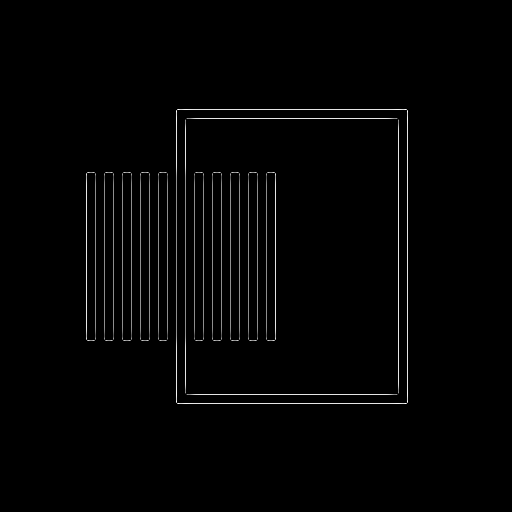
\includegraphics[width=.9\textwidth]{./canny/kanizsa_L2_a4_k11_k24}
    \caption{kanizsa, Isotropic L2 norm. $\alpha$ = 4, K1 = 1, K2 = 4}
    \label{fig:kanizsa_L2_a4_k11_k24}
  \end{subfigure}\\%
 \end{figure}

\begin{figure}[H]
\centering 
  \begin{subfigure}{.7\textwidth}
    \centering
    
\includegraphics[width=.9\textwidth]{./canny/kanizsa_ANISO_a4_k11_k24}
    \caption{kanizsa, Anisotropic. $\alpha$ = 4, K1 = 1, K2 = 4}
    \label{fig:kanizsa_ANISO_a4_k11_k24}
  \end{subfigure}%
  
\end{figure}
\subsubsection{kanisza, alpha = 5}
% Kanizsa, alpha = 2
\begin{figure}[H]
  \centering
  
    \begin{subfigure}{.7\textwidth}
    \centering
    
\includegraphics[width=.9\textwidth]{./canny/kanizsa_LINF_a5_k11_k24}
    \caption{kanizsa, Isotropic L-infinity norm. $\alpha$ = 5, K1 = 1, K2 = 4}
    \label{fig:kanizsa_LINF_a5_k11_k24}
  \end{subfigure}%

\end{figure}

\begin{figure}[H]
\centering

  \begin{subfigure}{.7\textwidth}
    \centering
    
\includegraphics[width=.9\textwidth]{./canny/kanizsa_L1_a5_k11_k24}
    \caption{kanizsa, Isotropic L1 norm. $\alpha$ = 5, K1 = 1, K2 = 4}
    \label{fig:kanizsa_L1_a5_k11_k24}
  \end{subfigure}%
  
  \begin{subfigure}{.7\textwidth}
    \centering
    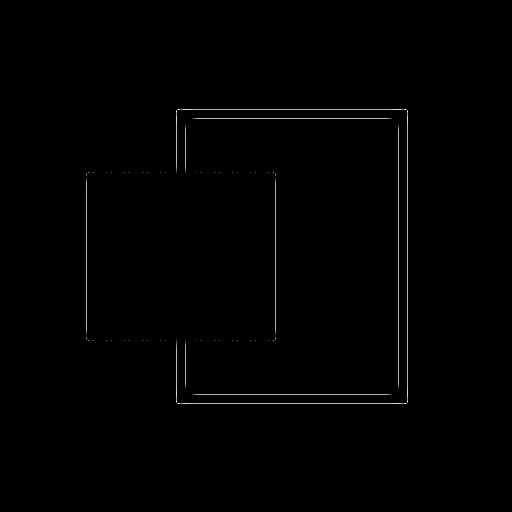
\includegraphics[width=.9\textwidth]{./canny/kanizsa_L2_a5_k11_k24}
    \caption{kanizsa, Isotropic L2 norm. $\alpha$ = 5, K1 = 1, K2 = 4}
    \label{fig:kanizsa_L2_a5_k11_k24}
  \end{subfigure}\\%
 \end{figure}

\begin{figure}[H]
\centering 
  \begin{subfigure}{.7\textwidth}
    \centering
    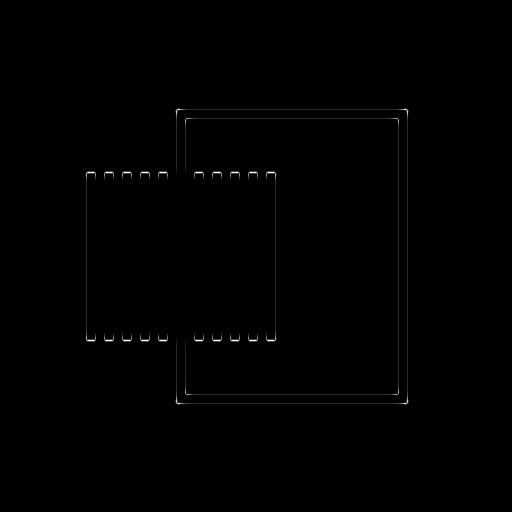
\includegraphics[width=.9\textwidth]{./canny/kanizsa_ANISO_a5_k11_k24}
    \caption{kanizsa, Anisotropic. $\alpha$ = 5, K1 = 1, K2 = 4}
    \label{fig:kanizsa_ANISO_a5_k11_k24}
  \end{subfigure}%
  
\end{figure}

\subsection{popout}
\begin{figure}[H]
  \centering
	\begin{subfigure}{.7\textwidth}
    \centering
    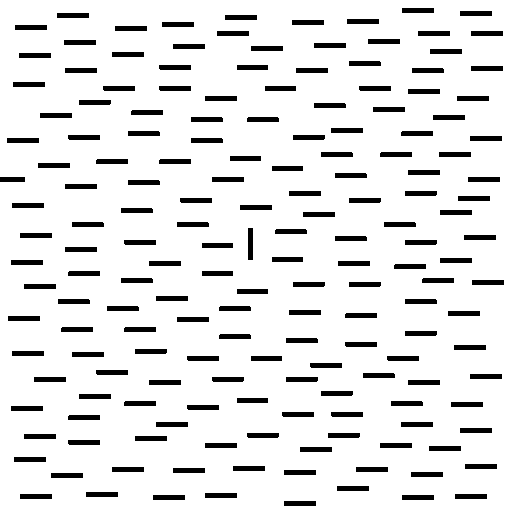
\includegraphics[width=.9\textwidth]{./canny/popout}
    \caption{Original popout image}
    \label{fig:popout}
  \end{subfigure}%    

\end{figure}
\subsubsection{popout, alpha = 3}
% popout, alpha = 2
\begin{figure}[H]
  \centering
	\begin{subfigure}{.7\textwidth}
    \centering
    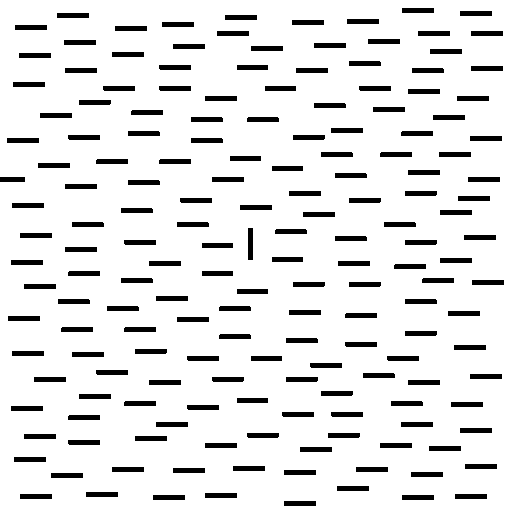
\includegraphics[width=.9\textwidth]{./canny/popout}
    \caption{Original popout image}
    \label{fig:popout}
  \end{subfigure}%    
  
    \begin{subfigure}{.7\textwidth}
    \centering
    \includegraphics[width=.9\textwidth]{./canny/popout_LINF_a3_k11_k24}
    \caption{popout, Isotropic L-infinity norm. $\alpha$ = 3, K1 = 1, K2 = 4}
    \label{fig:popout_LINF_a3_k11_k24}
  \end{subfigure}%

\end{figure}

\begin{figure}[H]
\centering

  \begin{subfigure}{.7\textwidth}
    \centering
    \includegraphics[width=.9\textwidth]{./canny/popout_L1_a3_k11_k24}
    \caption{popout, Isotropic L1 norm. $\alpha$ = 3, K1 = 1, K2 = 4}
    \label{fig:popout_L1_a3_k11_k24}
  \end{subfigure}%
  
  \begin{subfigure}{.7\textwidth}
    \centering
    \includegraphics[width=.9\textwidth]{./canny/popout_L2_a3_k11_k24}
    \caption{popout, Isotropic L2 norm. $\alpha$ = 3, K1 = 1, K2 = 4}
    \label{fig:popout_L2_a3_k11_k24}
  \end{subfigure}\\%
 \end{figure}

\begin{figure}[H]
\centering 
  \begin{subfigure}{.7\textwidth}
    \centering
    \includegraphics[width=.9\textwidth]{./canny/popout_ANISO_a3_k11_k24}
    \caption{popout, Anisotropic. $\alpha$ = 3, K1 = 1, K2 = 4}
    \label{fig:popout_ANISO_a3_k11_k24}
  \end{subfigure}%
  
\end{figure}
\subsubsection{popout, alpha = 4}
% Popout, alpha = 4

\begin{figure}
  \centering
    \makebox[\textwidth]{\includegraphics{./canny/popout_LINF_a4_k11_k24}} \\
  \caption{popout, Isotropic L-infinity norm. $\alpha$ = 3, K1 = 1, K2 = 4}
  \label{fig:popout_LINF_a4_k11_k24}
\end{figure}

\begin{figure}
  \centering
    \makebox[\textwidth]{\includegraphics{./canny/popout_L1_a4_k11_k24}} \\
  \caption{popout, Isotropic L1 norm. $\alpha$ = 3, K1 = 1, K2 = 4}
  \label{fig:popout_L1_a4_k11_k24}
\end{figure}

\begin{figure}
  \centering
    \makebox[\textwidth]{\includegraphics{./canny/popout_L2_a4_k11_k24}} \\
  \caption{popout, Isotropic L2 norm. $\alpha$ = 3, K1 = 1, K2 = 4}
  \label{fig:popout_L2_a4_k11_k24}
\end{figure}

\begin{figure}
  \centering
    \makebox[\textwidth]{\includegraphics{./canny/popout_ANISO_a4_k11_k24}} \\
  \caption{popout, Anisotropic. $\alpha$ = 3, K1 = 1, K2 = 4}
  \label{fig:popout_ANISO_a4_k11_k24}
\end{figure}

\end{document}